\documentclass[conference]{IEEEtran}
\IEEEoverridecommandlockouts
\usepackage{cite}
\usepackage{amsmath,amssymb}
\usepackage{graphicx}
\usepackage{booktabs}
\usepackage{multirow}
\usepackage{xcolor}
\usepackage{tikz}
\usetikzlibrary{arrows.meta,positioning,fit,calc}
\usepackage[hidelinks]{hyperref}
\usepackage{url}
\graphicspath{{figures/}}

\begin{document}

\title{Answer Only When the Radar Agrees: Calibrated Abstention for Plain-Language Flood Questions on Sentinel-1}

\author{
\IEEEauthorblockN{Sai Bhuwan S, Yashita Mandavilli, Raj Venkat, Nikhil S Rao, Shashwat Mittal, Sasanuru Anirudh}
\IEEEauthorblockA{Department of Computer Science and Engineering\\
RV Institute of Technology and Management, Bengaluru, India\\
Code and data: \url{https://github.com/UnKnownnPasta/satclip}}
}

\maketitle

\begin{abstract}
Vision-language assistants for remote sensing answer fluently but localise, count and handle radar poorly, and none of them tells a non-expert when not to trust an answer. We present EvidEO, an open, CPU-only system that answers plain-language questions about floods in Indian districts with an \emph{evidence card}: an area measured from the actual Sentinel-1 scene by a transparent instrument, the scene identifiers and dates, a mask, a calibrated confidence, and a receipt that re-runs to an identical output hash. Below a stated confidence the system abstains instead of guessing. We evaluate at the level of the answer a user receives, not the pixel. On the held-out Sen1Floods11 test split, publishing only answers with calibrated confidence of at least 0.60 cuts the share of wrong area answers from 45\% to 26\% while answering 43\% of questions. Leave-one-event-out analysis shows that a calibration fitted on other regions is systematically over-confident on South Asian monsoon events (India $+20$, Pakistan $+29$, Sri Lanka $+10$ points), so an assistant calibrated globally would publish half of its Indian answers with more than half of them wrong. Re-fitting only the intercept on as few as eight local labelled chips removes the over-confidence, but honest coverage on Indian chips then falls to about 13\%. For flood change, regime-specific calibration lowers expected calibration error from 0.255 to 0.041 and exposes that positive change answers are right only 27\% of the time. The lesson is that trustworthy assistants need local calibration data and better instruments more than larger language models. All eight receipts in our end-to-end demo re-ran to identical outputs.
\end{abstract}

\begin{IEEEkeywords}
Sentinel-1, flood mapping, visual question answering, calibration, selective prediction, abstention, provenance, domain shift
\end{IEEEkeywords}

\section{Introduction}

A district disaster official in Assam during the monsoon has a short, local question: how much of my district is under water since the last pass, and is it spreading? The answer exists in free Sentinel-1 radar data, but getting to it needs sensor knowledge, data wrangling and GIS skills. India's task force on geospatial education estimated 25{,}000 to 50{,}000 trained users against a need of about 500{,}000 more~\cite{ntfge2013}. Central agencies produce excellent flood products, about 300 in 2024 for the whole country~\cite{india2025copuos,nrsc2023atlas}, but central production cannot answer every official's own polygon and dates on demand. Optical imagery is of little help: cloud cover exceeds 60\% over most of India from June to September~\cite{shang2018monsoon}.

Remote-sensing vision-language models (RS-VLMs) such as GeoChat~\cite{kuckreja2024geochat}, EarthGPT~\cite{zhang2024earthgpt}, LHRS-Bot~\cite{muhtar2024lhrsbot} and EarthDial~\cite{soni2025earthdial} promise exactly this kind of plain-language access. Benchmarks, however, show that they are weakest where officials need precision (Fig.~\ref{fig:landscape}). GPT-4V localises the referred object at IoU 0.5 only 7.6\% of the time on DIOR-RSVG, against 76.8\% for a supervised specialist~\cite{zhang2024vleo}; on GEOBench-VLM the best referring-expression score is 34\%~\cite{danish2025geobench}; experts judge only 36\% to 68\% of remote-sensing VLM answers free of hallucination (69\% for the best general model)~\cite{zhou2026rshallu}. None of these systems attaches a calibrated probability to an answer or declines to answer when evidence is weak. A fluent wrong area figure is worse than no figure, because people rely on automation in proportion to how confident it appears~\cite{lee2004trust}.

We therefore invert the usual design. In EvidEO, \emph{instruments answer and the language model only asks and explains}: a versioned SAR water instrument produces every number, a calibration map turns its quality score into a probability that the published area is within tolerance, and the system abstains below a threshold. Our contributions are:
\begin{enumerate}
\item An open, CPU-only evidence-card system on public STAC catalogues~\cite{stac2024} and Cloud Optimized GeoTIFFs~\cite{ogc2023cog}, with automatic SAR selection under monsoon cloud and receipts that reproduce bit-for-bit (Section~\ref{sec:system}).
\item An \emph{answer-level} evaluation protocol for area questions, using risk-coverage curves and calibration error on hand-labelled flood chips from Sen1Floods11~\cite{bonafilia2020sen1floods11} and Kuro Siwo~\cite{bountos2024kurosiwo} (Section~\ref{sec:protocol}).
\item Evidence that answer calibration does not transfer geographically: a global fit is over-confident on every South Asian event in Sen1Floods11, and a few local labels fix the over-confidence at a large, honest cost in coverage (Section~\ref{sec:results}).
\end{enumerate}
We do not claim a better flood detector; our detector performs at the level of the published Otsu baseline (Table~\ref{tab:iou}). The claim is about what an assistant should say, and when it should say nothing.

\begin{figure*}[t]
\centering
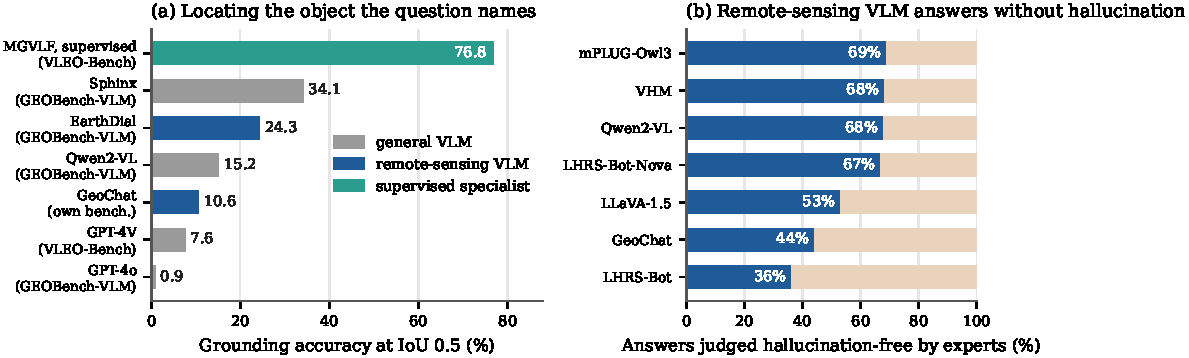
\includegraphics[width=\textwidth]{fig_landscape.pdf}
\caption{What the literature reports, re-plotted from the papers' own tables. (a) Referring or grounding accuracy at IoU 0.5: GPT-4V, MGVLF on DIOR-RSVG~\cite{zhang2024vleo}; GPT-4o, Qwen2-VL, EarthDial, Sphinx on GEOBench-VLM referring detection~\cite{danish2025geobench}; GeoChat on its own referring benchmark~\cite{kuckreja2024geochat}. Benchmarks differ, so bars compare orders of magnitude, not ranks. (b) Expert-judged hallucination-free rate on RSHalluEval, 300 sampled answers per model~\cite{zhou2026rshallu}; mPLUG-Owl3, Qwen2-VL and LLaVA-1.5 are general models.}
\label{fig:landscape}
\end{figure*}

\section{Related Work}

\textbf{RS vision-language models.} RSVQA~\cite{lobry2020rsvqa} framed questions over imagery; VRSBench~\cite{li2024vrsbench} and GEOBench-VLM~\cite{danish2025geobench} broadened the tasks. GeoChat~\cite{kuckreja2024geochat} reports 90.7\% on RSVQA-LR (whose training questions are in its instruction set) yet 10.6\% referring accuracy; EarthDial~\cite{soni2025earthdial} adds multispectral and SAR inputs and reaches 69.9\% on BigEarthNet. Pixel-grounded reasoners such as TerraScope~\cite{shu2026terrascope} return masks with answers and, given both optical and SAR inputs, learn to favour SAR over clouded regions. None reports calibrated per-answer confidence, and benchmarks either delete uncertain questions or count refusals as errors~\cite{zhang2024vleo,li2024vrsbench}.

\textbf{EO agents.} Tool-using agents route questions to code and models: OpenEarthAgent~\cite{shabbir2026openearthagent} replays tool traces, UnivEARTH agents~\cite{kao2026univearth} fetch live data, and EO-Gym~\cite{ma2026eogym} learns to switch to SAR. They improve grounding but leave the final answer's reliability unstated. RSure-Agent~\cite{rsure2026} lets tools return an ``insufficient evidence'' observation with a reason, but has no confidence threshold and answers through hosted models; an onboard multi-agent pipeline~\cite{onboard2026} runs a small VLM and LLM entirely on a CPU-only space-qualified board, showing that CPU-only analysis is feasible.

\textbf{Reliability in EO.} SHRUG-FM~\cite{gonzalez2026shrug} is the closest work: it rejects unreliable flood segmentations from a foundation model and reports a flood AURC of 0.115 on WorldFloods (Sentinel-2), with scores its authors deliberately leave uncalibrated and a binary hand-off to a human reviewer. The Copernicus Global Flood Monitoring product combines three SAR algorithms into a per-pixel ensemble likelihood with an exclusion layer for areas it cannot map~\cite{krullikowski2023gfm}; the likelihood is not fitted to labels and its reliability is shown only qualitatively. Classic SAR flood chains use split-based automatic thresholding~\cite{martinis2009split,twele2016s1flood}. From general ML we borrow Platt scaling~\cite{platt2000probabilities}, calibration error~\cite{guo2017calibration}, selective classification~\cite{geifman2017selective} and conformal methods~\cite{angelopoulos2021raps}. Our difference is the unit of evaluation: the area answer a non-expert reads, and the transfer of its calibration to a new region.

\section{System}
\label{sec:system}

\begin{figure}[t]
\centering
\resizebox{\columnwidth}{!}{%
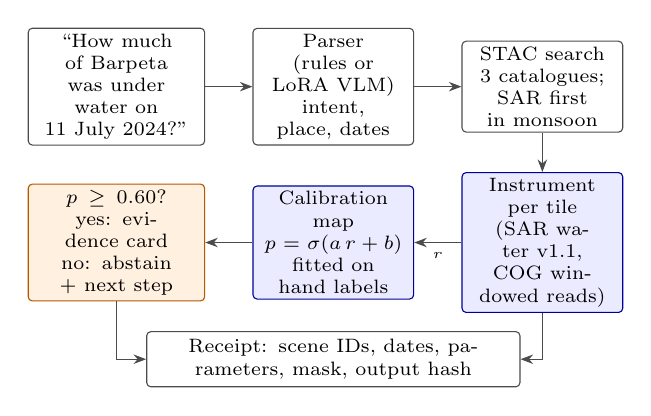
\begin{tikzpicture}[
  node distance=3mm and 6mm,
  box/.style={draw=black!70, rounded corners=1.5pt, align=center, font=\scriptsize, minimum height=7mm, inner sep=2pt, fill=white},
  key/.style={box, fill=blue!8, draw=blue!60!black},
  gate/.style={box, fill=orange!12, draw=orange!70!black},
  arr/.style={-{Stealth[length=1.6mm]}, draw=black!70}]
\node[box, text width=21mm] (q) {``How much of Barpeta\\was under water on\\11 July 2024?''};
\node[box, right=of q, text width=19mm] (p) {Parser (rules or\\LoRA VLM)\\intent, place, dates};
\node[box, right=of p, text width=19mm] (s) {STAC search\\3 catalogues;\\SAR first in monsoon};
\node[key, below=5mm of s, text width=19mm] (i) {Instrument per tile\\(SAR water v1.1,\\COG windowed reads)};
\node[key, left=of i, text width=19mm] (c) {Calibration map\\$p=\sigma(a\,r+b)$\\fitted on hand labels};
\node[gate, left=of c, text width=21mm] (g) {$p \ge 0.60$?\\yes: evidence card\\no: abstain + next step};
\node[box, below=4mm of c, text width=46mm] (r) {Receipt: scene IDs, dates, parameters, mask, output hash};
\draw[arr] (q) -- (p); \draw[arr] (p) -- (s); \draw[arr] (s) -- (i);
\draw[arr] (i) -- node[below, font=\tiny]{$r$} (c); \draw[arr] (c) -- (g);
\draw[arr] (i.south) |- (r.east); \draw[arr] (g.south) |- (r.west);
\end{tikzpicture}}
\caption{EvidEO answer path. Every number comes from an instrument; the language layer only parses the question and phrases the card.}
\label{fig:arch}
\end{figure}

\textbf{Question parsing.} A rule parser with a gazetteer of 735 Indian districts (geoBoundaries, ODbL) maps a question to one of four supported intents (water extent, water change, vegetation change, land description), a district and a date window; anything else is refused. A LoRA pipeline for Qwen2-VL-2B is provided as an optional parser and explainer; it never produces numbers. On 44 hand-written questions never used for tuning, the rule parser matches all fields on 68\%.

\textbf{Data.} The system searches Element84 Earth Search, Microsoft Planetary Computer and the Copernicus Data Space Ecosystem through STAC, with fail-over. In monsoon months (June to September) water questions go to Sentinel-1 first. Pixels are read as windowed COG reads per 0.05$^\circ$ tile and resampled to a 20~m working grid in NumPy rather than through GDAL decimation, which we found to be non-deterministic under concurrent reads.

\textbf{Instrument.} SAR water v1.1 follows the split-based approach of Martinis et al.~\cite{martinis2009split}, used in operational Sentinel-1 chains~\cite{twele2016s1flood}: each tile is split into 1~km blocks, blocks whose Otsu split~\cite{otsu1979threshold} is clearly bimodal (Ashman $D\ge3$) are pooled, and a minimum-error threshold~\cite{kittler1986minimum} is fitted on the pool, separately for VV and VH (gamma0, dB, with plausibility bounds chosen on the training split only). A pixel is water if either polarisation is below its threshold. The raw quality score $r$ is the probability that the area stays within tolerance under a 1~dB threshold error, times an evidence factor for how bimodal the fit was (0.75 when a default threshold had to be used). A change instrument compares same-orbit before and after scenes.

\textbf{Calibration and abstention.} A Platt map~\cite{platt2000probabilities} $p=\sigma(a r+b)$ estimates the probability that the published area is correct (defined below). Tile results are aggregated with fully correlated uncertainty into a district card. Cards with $p<0.60$ abstain and offer the follow-up most likely to help (for a change question, the two single-date extents).

\textbf{Receipts and scale.} Each card stores scene IDs, acquisition dates, instrument version, parameters and a hash of the output raster. Work is split into tiles on a Redis queue with stateless workers. On two vCPUs a whole district (117 tiles) takes 77 to 98~s cold and 0.5~s from cache; with 400~ms simulated read latency, throughput scales from 2.0 to 7.8 tiles/s going from one to four workers.

\begin{figure}[t]
\centering
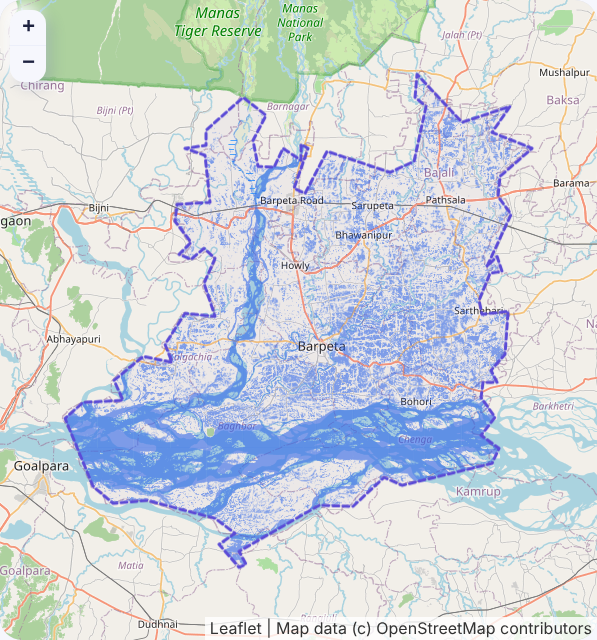
\includegraphics[width=0.49\columnwidth]{fig_barpeta_map.png}\hfill
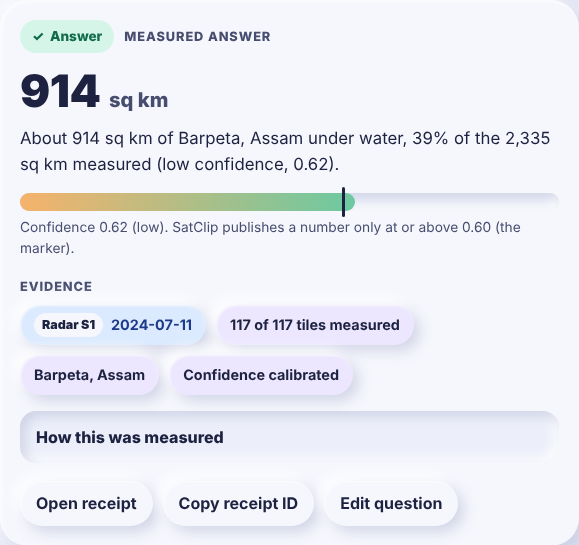
\includegraphics[width=0.49\columnwidth]{fig_card.png}
\caption{Prototype on live data: Barpeta, Assam, Sentinel-1 pass of 11 July 2024. Left: measured water per tile over the district outline. Right: the published card (914 km$^2$, confidence 0.62, scene and date chips, receipt). The figure includes the Brahmaputra channel and permanent wetlands; it is water extent, not verified flood extent.}
\label{fig:demo}
\end{figure}

\section{Answer-Level Evaluation Protocol}
\label{sec:protocol}

Pixel IoU does not tell a user whether the number on the card is usable. We call an area answer \emph{correct} when the measured water area is within $\pm 20\%$ of the hand-labelled area, with a floor of 5\% of the valid chip area so that near-empty chips are not judged on noise. We then report: share correct when always answering; expected calibration error (ECE, 10 bins)~\cite{guo2017calibration}; coverage (share of questions answered) and risk (share of published answers that are wrong) at the 0.60 threshold; and the area under the risk-coverage curve (AURC)~\cite{geifman2017selective}.

\textbf{Water extent data.} Sen1Floods11 hand-labelled chips~\cite{bonafilia2020sen1floods11}: 408 of 446 usable (at least half the chip valid and labelled), from 11 events in 11 countries. The calibration map is fitted on the train and valid splits (312 chips) and tested on the test split (82) and the held-out Bolivia event (14). For transfer, we run leave-one-event-out (LOEO): fit on all other events, test on the held-out one.

\textbf{Water change data.} Kuro Siwo~\cite{bountos2024kurosiwo}: 848 before and after samples from 22 events, evaluated with 5-fold cross-validation grouped by event.

\section{Results}
\label{sec:results}

\begin{table}[t]
\centering
\caption{Detector sanity check: mean per-chip IoU of the water class on Sen1Floods11. Published values from~\cite{bonafilia2020sen1floods11}, Tables 1 and 2 (all-water column). Protocols differ slightly (we resample to 20~m and drop chips under 50\% valid).}
\label{tab:iou}
\begin{tabular}{lcc}
\toprule
Method & Test & Bolivia \\
\midrule
Otsu-VH thresholding (published) & 0.359 & 0.386 \\
Best FCN-ResNet50, S1 input (published) & 0.408 & 0.387 \\
EvidEO SAR water v1.1 (ours) & 0.362 & 0.434 \\
\bottomrule
\end{tabular}
\end{table}

\textbf{The detector is ordinary.} Table~\ref{tab:iou} confirms that our instrument, a classic thresholding chain, performs at the published Otsu level. Everything below is therefore about how answers are gated, not about segmentation quality.

\begin{figure}[t]
\centering
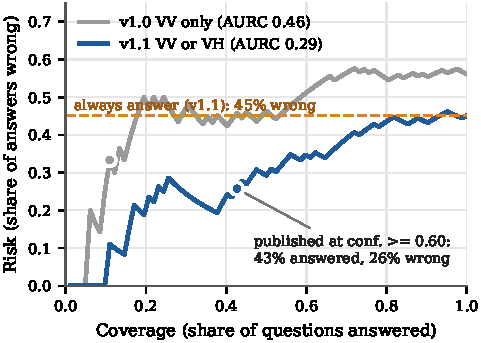
\includegraphics[width=\columnwidth]{fig_riskcov.pdf}
\caption{Risk-coverage on the held-out Sen1Floods11 test split (82 chips). Answers are sorted by calibrated confidence; the dot marks the 0.60 publishing threshold. Oracle AURC is 0.125 (v1.1); random ordering gives 0.451.}
\label{fig:rc}
\end{figure}

\textbf{Abstention makes published answers more reliable.} Always answering, 45.1\% of area answers on the test split are wrong (Fig.~\ref{fig:rc}). Publishing only at $p\ge0.60$ answers 42.7\% of questions with 25.7\% wrong (95\% bootstrap interval 11.9\% to 41.0\%). Calibration lowers ECE from 0.139 to 0.074. Adding VH (v1.1) improves the ranking itself: AURC falls from 0.457 to 0.289, and coverage at the threshold rises from 11\% to 43\%. For orientation only, SHRUG-FM reports a flood AURC of 0.115~\cite{gonzalez2026shrug} on a different dataset, sensor and failure definition, and our oracle bound here is 0.125; the numbers are not comparable head to head.

\begin{figure}[t]
\centering
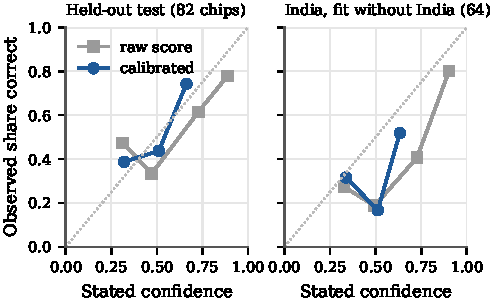
\includegraphics[width=\columnwidth]{fig_reliability.pdf}
\caption{Reliability diagrams (5 bins, bins with at least 3 chips). Left: test split. Right: the 64 Indian chips with a map fitted without India; calibrated confidence near 0.5 corresponds to under 20\% correct.}
\label{fig:rel}
\end{figure}

\begin{figure}[t]
\centering
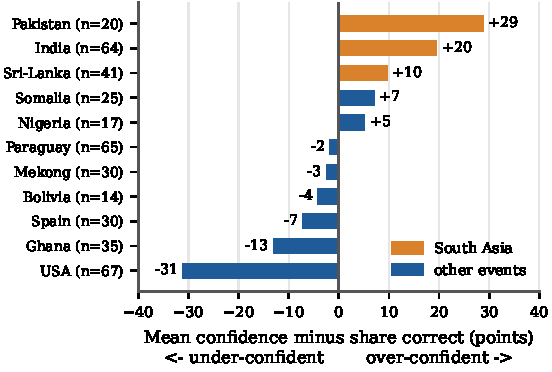
\includegraphics[width=\columnwidth]{fig_loeo.pdf}
\caption{Calibration transfer, leave one event out. Bars show mean calibrated confidence minus the observed share correct on the held-out event. All three South Asian events are over-confident.}
\label{fig:loeo}
\end{figure}

\textbf{Calibration does not travel.} Fig.~\ref{fig:loeo} shows that a map fitted on other regions is over-confident on India by 20 points, Pakistan by 29 and Sri Lanka by 10, and under-confident on the USA by 31. For India this means 52\% of chips would be published with 55\% of those wrong (Table~\ref{tab:sel}), worse than the test split's unfiltered error. Within India the raw score still ranks answers better than chance (AUROC 0.65), so the failure is mostly an offset, not a reversal. We cannot isolate the cause from these data; plausible contributors are paddy and wet soil with low backscatter, vegetated and urban flooding, and terrain, which a planned version will mask with HAND. A recent study of 19 unseen flood events found detection near zero under tree cover and in built-up areas but far better on cropland and riverine floods~\cite{kolluru2026limits}, which suggests calibrating offsets per land-cover and flood-type regime rather than per region.

\begin{table}[t]
\centering
\caption{Answer-level results for water extent at the 0.60 threshold.}
\label{tab:sel}
\setlength{\tabcolsep}{3.2pt}
\begin{tabular}{lccccc}
\toprule
Evaluation set & $n$ & Always-answer & ECE & Coverage & Risk \\
 & & error & & & \\
\midrule
Test split & 82 & 0.45 & 0.074 & 0.43 & 0.26 \\
Bolivia (unseen country) & 14 & 0.43 & 0.323 & 0.43 & 0.00 \\
India, global map (LOEO) & 64 & 0.64 & 0.247 & 0.52 & 0.55 \\
India, 8 local chips$^\dagger$ & 56 & 0.64 & 0.164 & 0.13 & 0.28 \\
\bottomrule
\multicolumn{6}{l}{\footnotesize $^\dagger$Intercept-only refit, mean of 500 random splits; risk over runs that publish.}
\end{tabular}
\end{table}

\begin{figure*}[t]
\centering
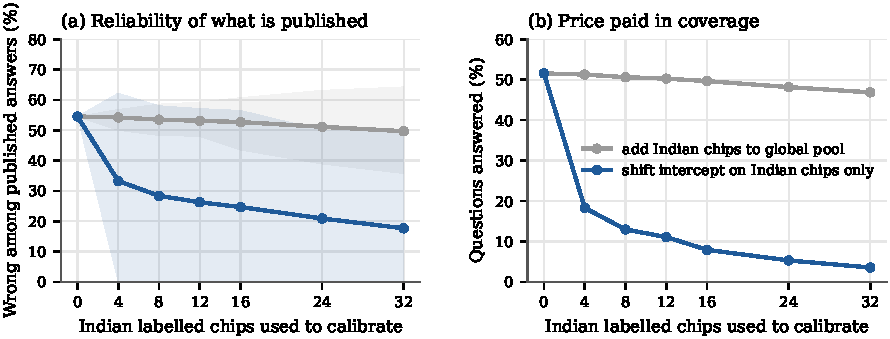
\includegraphics[width=\textwidth]{fig_local.pdf}
\caption{How many local labels does trust need? Indian chips are split at random 500 times into $k$ calibration chips and the rest for evaluation. Grey: add the $k$ chips to the global fitting pool (the global data swamp them). Blue: keep the global slope and refit only the intercept on the $k$ local chips. Bands are 10th to 90th percentiles; with few published answers per run the lower band reaches zero.}
\label{fig:local}
\end{figure*}

\textbf{A few local labels restore honesty, and reveal the true coverage.} Fig.~\ref{fig:local} compares two ways of using $k$ labelled Indian chips. Pooling them with the global data barely moves anything. Refitting only the intercept removes the over-confidence with four to eight chips (mean offset from $+20$ to under 1 point at $k=8$) and lowers the share of wrong published answers from 55\% to 28\%, falling to 18\% at $k=32$. The price is coverage: the honest system answers about 13\% of Indian questions at $k=8$ and abstains on the rest, and in about 40\% of random splits it publishes nothing. We consider this the correct behaviour. The instrument is weak on these chips, and the calibrated system says so instead of hiding it.

\begin{figure}[t]
\centering
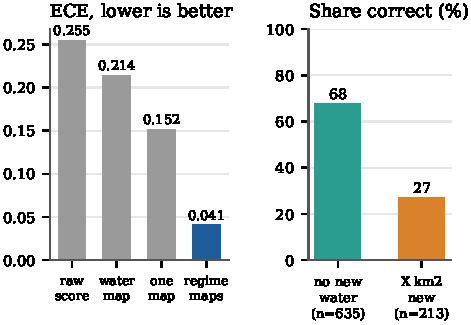
\includegraphics[width=\columnwidth]{fig_change.pdf}
\caption{Water change on Kuro Siwo (848 samples, 22 events, grouped 5-fold CV). Left: ECE of four calibration maps. Right: the two answer types differ sharply in reliability, which is why separate maps per regime are needed.}
\label{fig:change}
\end{figure}

\textbf{Change answers need regimes.} For flood change, the raw score barely separates right from wrong answers (AUROC 0.52) because two kinds of answer are mixed (Fig.~\ref{fig:change}). ``No meaningful new water'' answers are right 68\% of the time; ``X km$^2$ of new water'' answers only 27\%, mostly by undercounting (75\% undercount by more than 20\%). Fitting one map per answer regime lowers ECE from 0.255 to 0.041 and raises AUROC to 0.64. In practice the change card abstains on almost every positive change answer and offers the two single-date extents instead; in our live Barpeta demo it abstained at 0.23 and the follow-ups published 413 and 914~km$^2$.

\textbf{Receipts reproduce.} All eight cards of the scripted demo (713 tiles over Barpeta and Darbhanga) re-ran from a cold cache to identical receipt identifiers and output hashes.

\section{Discussion and Limitations}

\textbf{What this shows.} Answer-level calibration is cheap and turns a mediocre detector into an assistant whose published numbers can be relied on at a stated rate. It also shows that the bottleneck for Indian flood questions is local labels and instrument quality, not language modelling: the same over-confidence would afflict any RS-VLM that states confidence without regional calibration.

\textbf{Limitations.} (1) Sample sizes are small. The 64 Indian chips come from one Sen1Floods11 event and are spatially correlated, so Fig.~\ref{fig:local} measures within-event transfer; the bootstrap interval on test risk is wide. (2) The $\pm20\%$ tolerance is our choice; we have not validated it with officials. (3) District cards aggregate tiles with an assumed correlation, and the calibration was fitted on 5~km chips. (4) The Barpeta figure includes permanent water and has not been compared with NRSC maps. (5) We did not run RS-VLMs on the same area questions; Fig.~\ref{fig:landscape} compares across benchmarks. (6) No user study yet tests whether non-experts read cards correctly; this is the most important missing evidence. (7) The vegetation-change instrument has no fitted calibration and is labelled as such on its cards.

\textbf{Next steps.} Mask terrain with HAND and permanent water with the Sentinel-1 archive, add per-pixel water probabilities, gather labelled chips from several Indian events (for example Assam and Bihar) to test across-event transfer, replace the fixed threshold with conformal risk control~\cite{angelopoulos2021raps}, and run a timed task study with non-GIS users.

\section{Conclusion}

An assistant that answers every question is easy to build and hard to trust. EvidEO answers plain-language flood questions with measured, receipted, calibrated evidence cards and abstains when the radar does not support an answer. Our experiments show that such abstention works on held-out data, that calibration fitted elsewhere is over-confident on South Asian floods, and that a handful of local labels fixes the confidence while revealing how much the instrument can honestly answer. We release the system, the per-chip results and the analysis scripts so that others can test their assistants at the level of the answer.

\section*{Acknowledgment}
We thank the creators of Sen1Floods11 and Kuro Siwo for open hand-labelled data, and ESA Copernicus, Element84 and Microsoft Planetary Computer for open access to Sentinel data.

\bibliographystyle{IEEEtran}
\bibliography{refs}

\end{document}
